\chapter{$b$-tagging efficiency at high $p_{T}$}
\label{AppendixB}

One of the limiting factors of the signal acceptance in the $FourBfull$ search at high resonance masses is the degradation of the $b$-tagging efficiency for high $p_{T}$ jets. This appendix presents a study of the underlying causes of this degradation. 

\section{MV2 algorithm overview}

The MV2 algorithm is a boosted decision tree incorporating twenty-four input variables constructed from three lower level input algorithms: IPxD, SV1, and JetFitter. IPxD uses the two and three dimensional impact parameter information of tracks in the jet to construct templates for light, charm, and bottom quarks and compute likelihood ratios. SV1 is a secondary vertex reconstruction algorithm. JetFitter atemtps to fit to the full decay chain of the $B$ hadron, looking for multiple decay vertices aligned along a single axis. Figure~\ref{fig:MV2inputs} summarizes the inputs to MV2. 

\begin{figure}[h!]
  %\vspace{20pt}
  \centering
  \captionsetup{justification=centering}

  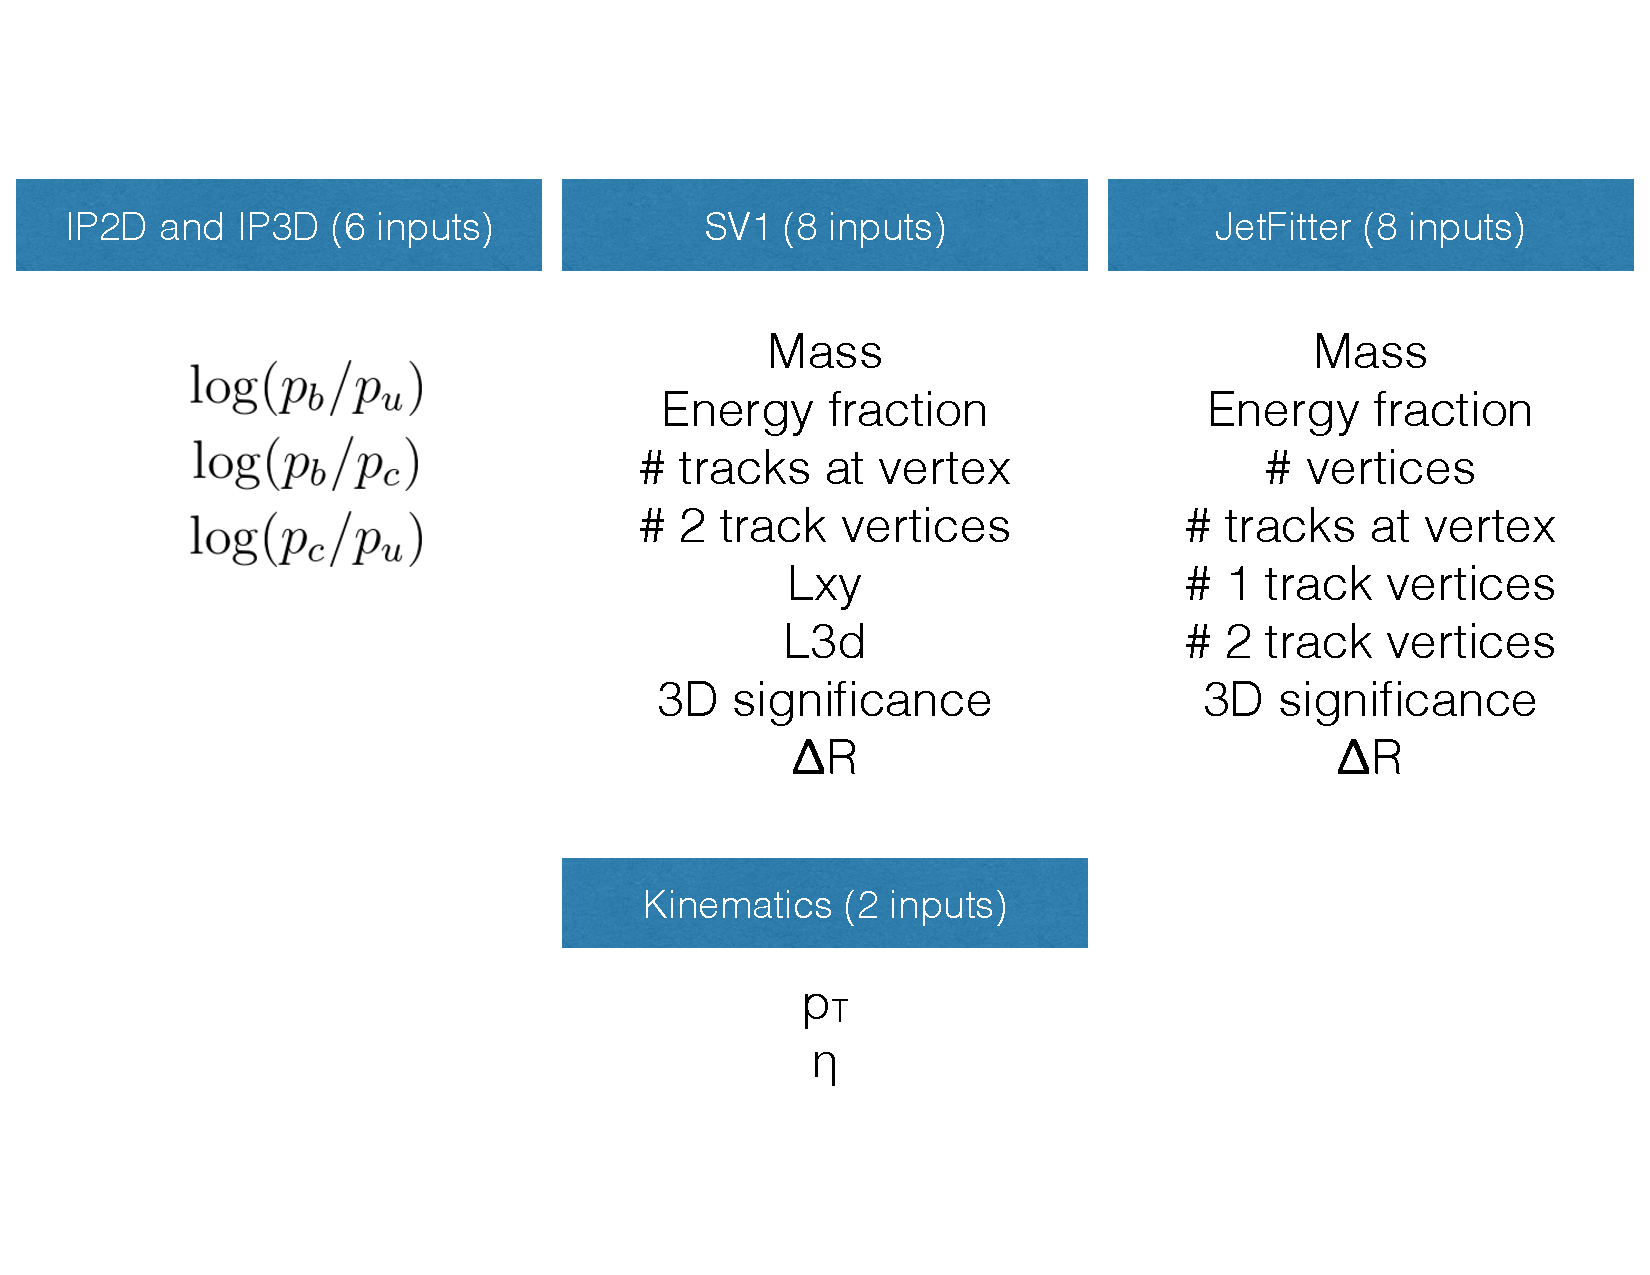
\includegraphics[width=0.7\textwidth]{figures/MV2_inputs}
  \caption{Summary of the inputs to the MV2 $b$-tagging algorithm}
  \label{fig:MV2inputs}
\end{figure}

\section{Changes in MV2 score at high $\pT$}

The degradation of $b$-tagging at high $\pT$ was studied in particular in the context of RSG models at high mass. Figure~\ref{fig:TrackJetPt} shows the $\pT$ of the leading track jet inside of the leading calorimeter jet in RSG events. At high $m_{\Gkk}$, the $\pT$ spectrum of track jets is much harder than at lower masses due to the increased Higgs $\pT$. 

\begin{figure}[h!]
  %\vspace{20pt}
  \centering
  \captionsetup{justification=centering}

  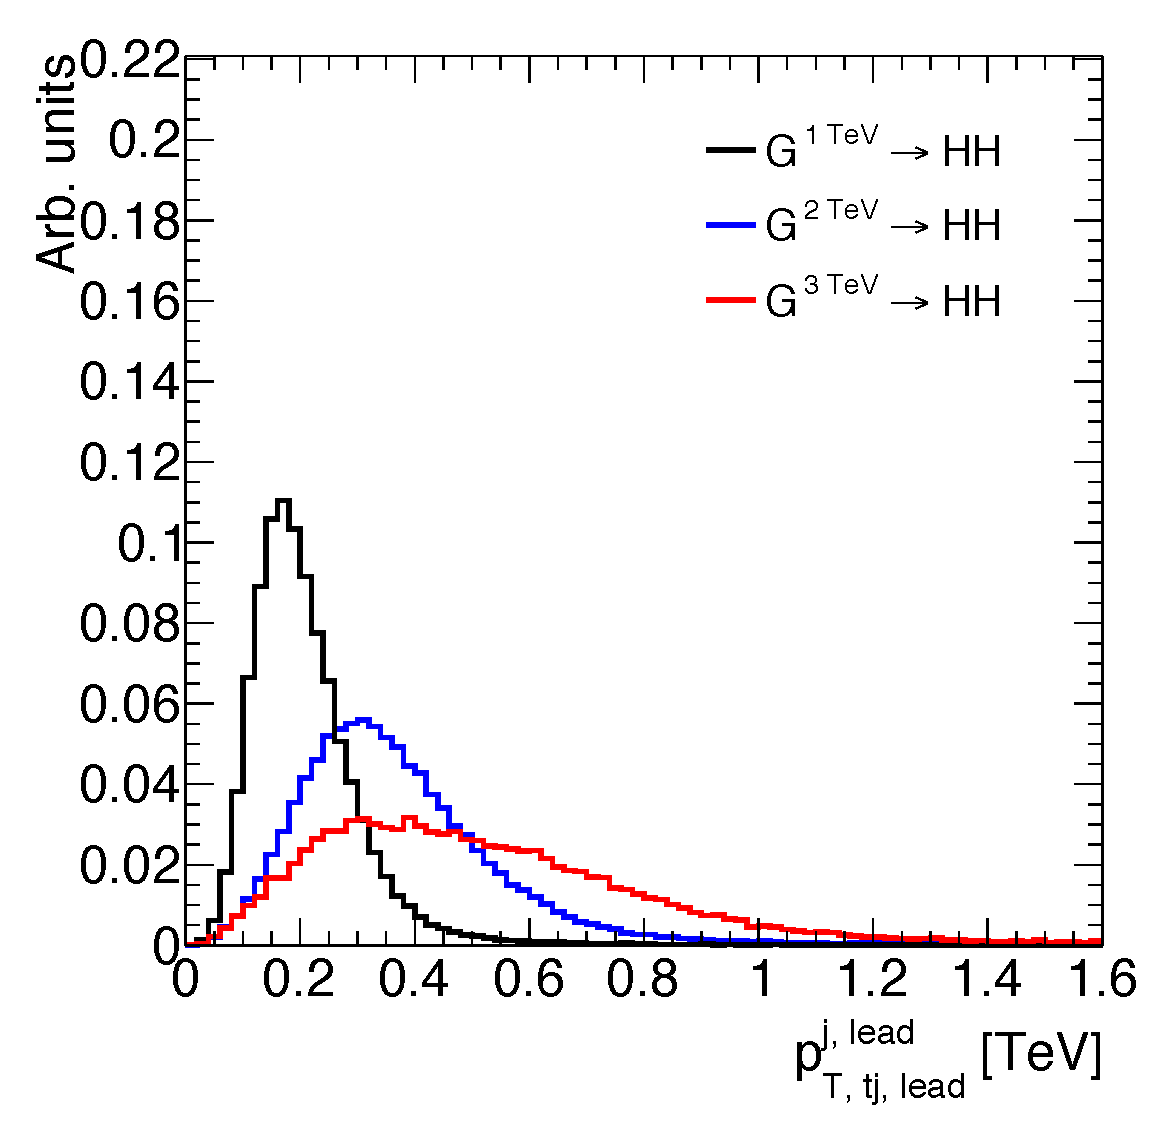
\includegraphics[width=0.6\textwidth]{figures/TrackJetPt}
  \caption{$\pT$ distribution for the leading track jet in the leading calorimeter jet for different signal masses in RSG $c=1$ models}
  \label{fig:TrackJetPt}
\end{figure}